
\chapter{Designing a Synchronization Framework}\label{main}

\section{Application Scenario: A Collaborative Task Manager}
Our goal is to develop a collaborative Task Manager that can still be used if disconnected from the network.
We choose this scenario because we think it represents a common type of architecture and data model for mobile applications.

Let us first work out some user stories and then try to define a suitable data model for such an application.

\subsection{User Story 1: Creating Projects}
\begin{itemize}
\item A User can create Projects in order to coordinate Tasks.
\item A User can invite other Users as Project Members to a Project.
\end{itemize}

Examples for Projects created by User Rita would be:\\

\begin{tabular}{ l l }
Project Name & Members \\
\hline
Marketing Material & Rita, Tom, Allen \\
Product Roadmap & Rita, Allen \\
Sales Review & Rita, Lisa
\end{tabular}

\subsection{User Story 2: Creating and Editing Tasks}
\begin{itemize}
\item Project Members can add Tasks to a Project in order to manage responsibilities.
\item A Task can have a due date and responsible project member assigned.
\item A Task can be edited by Project Members and marked as done.
\item A Task can be moved in the list of Tasks.
\end{itemize}

An example list of Tasks could be:\\

\begin{tabular}{ l l l l }
\multicolumn{4}{ c }{Project ``Marketing Material''} \\
Task & Due Date & Assignee & Done \\
\hline
Create event poster & 2013-08-12 & Rita & No\\
Write blog entry on event & 2013-07-20 & Tom & Yes
\end{tabular}

\subsection{User Story 3: Commenting on Tasks}
\begin{itemize}
\item Project Members can add Comments to Tasks
\end{itemize}

Examples would be:\\

\begin{tabular}{ l l l }
\multicolumn{3}{ c }{Task ``Create event poster'' in Project ``Marketing Material"} \\
Member & Date & Comment \\
\hline
Rita & 2013-07-20 & Allen, I need you to create some graphics. \\
Allen & 2014-07-20 & Ok, lets go through it tomorrow morning!
\end{tabular}

\subsection{User Story 3: User Workflows}
\begin{itemize}
\item In order to be productive a user needs to access all Tasks from any device.
\item A user should be able to Edit and Create Projects and Tasks when disconnected from any network.
\item The data should be kept as current as possible even if a user's device does not have reliable internet access.
\end{itemize}

An example workflow that should be supported:\\

\begin{itemize}
\item Rita works at the desktop computer in her office with high-speed internet access. She creates Project A and invites Allen.
\item Allen works from home on his notebook with high-speed internet access. He reviews the Project and creates task A1.
\item Rita is already on her way home but has mobile internet access on her smartphone. She receives the added task A1 and edits its title.
\item Rita is still on the train but decides to continue working on her notebook. Her notebook does not have internet access but she can establish a direct connection to her smartphone via Wifi. The reception on her smartphone has dropped in the meanwhile. She receives the latest updates from her smartphone and adds a comment to task A1.
\item Allen who is still at home can not receive Rita's comment as she is still on the train. In the meanwhile he creates a Task A2 in Project A.
\item Rite gets home where she has internet access with her notebook. She receives Allen's created Task A2.
\item Allen, who is still at his notebook, receives Rita's comment as soon as she connects to internet at home.
\end{itemize}

\subsection{Data Model}
Based on the user stories we can derive a plausible data model for the application. We can map it to an entity-relationship model as shown in figure \ref{fig:tasks-data-model}.\\
The only complication is the requirement of Tasks per Project being ordered. We model this as a linked list by having a ``Next Task'' relationship.

\begin{figure}[tasks-data-model]
\centering
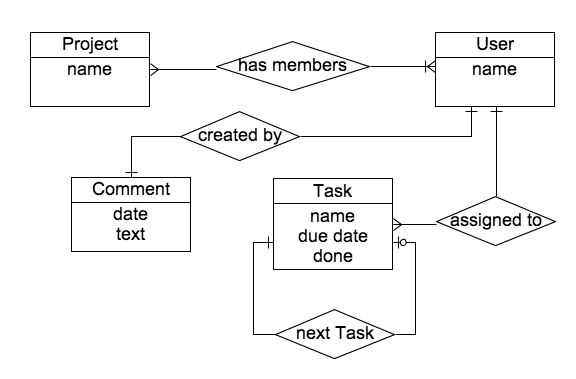
\includegraphics[width=0.8\textwidth]{img/tasks-schema}
\caption{A collaborative Task Manager's data model}
\label{fig:tasks-data-model}
\end{figure}

\section{Requirements}
\label{sec:requirements}
From the application scenarios we can derive a set of requirements for a synchronization solution.\\
The listed requirements resemble the goals set for the Bayou architecture back in 1994 \cite{Demers:1994vj}. 
Bayou had already proposed a distributed architecture with multiple devices acting as server.
At that time the computational capabilities of mobile devices were very limited.
Today even smartphones have more storage and stronger CPUs than most servers in 1994.
So pairwise synchronization should not only be possible between servers but also between mobile devices directly.

Phases of synchronization:
- Update Detection
- Update Propagation
- Reconciliation

\subsection{Flexible Data Model Support}
A synchronization engine that is useful for a broad range of applications has to be able to deal with different data models. There is no magic algorithm that produces a perfect solution for an existing application.
Synchronization can happen with increasing levels of sophistication depending on the amount of understanding of an application's data.\\
A ``dumb'' solution would have no understanding of an app's data model at all - it simply sees the entire application data as one binary chunk.\\
A more clever solution would maybe have an understanding of entities like Projects, Tasks or Comments and would see the entity instances as binary data.\\
It could get even finer grained and break up each entity instance into attributes which it recognizes as different pieces of data.\\
We see that \emph{synchronization granularity} is one key aspect when evaluating solutions.
The smallest pieces of information a syncing engine can not break up further we call \emph{atoms}.
Atoms are usually aggregated into larger structures we call \emph{objects}.
A Task instance could be treated as an object which composes the title and due date attributes as atoms.\\
In order to be useful a synchronization engine does not need perfect understanding of the data to be synchronized.
Popular applications like Dropbox can provide useful synchronization of files without having any semantic understanding of their content.
For Dropbox each file is an atom - if a user adds a paragraph to a Word document, Dropbox only recognizes a change to the entire file.
This means if two users concurrently modify the same document at different places, Dropbox has no way to merge the changes correctly and will trigger a conflict.\\
Version control systems like git are usually more sophisticated - git treats each line in a file as an atom and can therefore often successfully merge concurrent changes.
Git still does not have any syntactic or even semantic understanding of the code that is written in the files it synchronizes.
So if there are concurrent edits, git can not guarantee that merges are synctactically or semantically correct.
Despite this git is useful enough to be used very successfully in large software projects.\\

We therefore need to evaluate carefully how much semantic understanding of an application's data a synchronization engine actually needs to be useful.

The data model of our application scenario is relatively simple but covers most of the modeling aspects an average mobile application needs:

\begin{itemize}
\item Entities and Instances
\item (Ordered) Collections
\item Attributes
\item Relationships (one to one, one to many, many to many)
\end{itemize}

This set of modeling elements is represented in many client-side application frameworks like Ember.js, Backbone or Angular.
If we can support synchronizing data with this type of schema it will make integration with existing frameworks fairly trivial.

\subsection{Optimistic Synchronization}
As we have seen in the application scenario it is necessary that objects are editable on multiple devices even if they are not connected to a network.
Edits should be allowed concurrently to not block users from doing their work.
This implies that there can not be a central locking mechanism that controls when users can synchronize their data for offline usage.
We therefore trade strict consistency for availability of the data.\\
Synchronization happens in an optimistic manner which means that we assume that temporarily inconsistent data will rarely lead to problems.

\subsection{Eventual Consistency}
The sequence of states an object goes through as its edited is called its \emph{history}.
The history forms a directed graph with each state except the intial state having at least one ancestor.
The \emph{current state} is the one that has no descendants.
As edits can be made on different devices concurrently there can be multiple \emph{current states} at a time.
If an object has multiple current states we refer to them as \emph{branches}.\\
Our goal is to guarantee that after a finite number of synchronization events the object will eventually converge to the same state across all devices.

\subsection{Causality Preservation and Conflicts}
If an object diverges into multiple branches it will have to be reconciled during the synchronization process.
When we receive states from a remote device we need to reason about how we can apply them to our own edit history.\\
The \emph{happens-before} relationship defined by Lamport in \cite{Lamport:1978tr} helps to reason about this problem in an intuitive way.
A state \emph{a} that \emph{happened before} state \emph{b} refers to the fact that the edits that led to \emph{b} could have been affected by \emph{a}.
It is not necessarily related to the actual time of the edits that led to \emph{a} and \emph{b} as we can see in the following example:\\

Lets assume Rita and Allen work on the same object with their respective devices.
The object has the initial state \emph{a}.

\begin{itemize}
\item 9:00 AM: Rita makes an edit to the object which leads to state \emph{b}.
\item 9:30 AM: Allen synchronizes with Rita and edits which leads to state \emph{c}.
\item 10:00 AM: Rita is offline and can not synchronize. She edits the object at state \emph{b} leading to state \emph{d}. 
\end{itemize}

As Allen has seen state \emph{b} when making his edit, state \emph{b} \emph{happened before} state \emph{c}.\\
Rita has not seen state \emph{c} when making her edit.
Although the time of her edit is after Allen's edit there is no \emph{happened-before} relationship between state \emph{c} and \emph{d}.\\
On the next synchronization between Allen and Rita the system needs to identify this lack of causality as a \emph{conflict}.\\
While this example is simple, the identification of conflicts among a large group of collaborators can be non-trivial.\\
Depending on the level of understanding the synchronization engine has on the data there are strategies to resolve conflicts automatically.
The engine should be designed in a way that conflict resolution strategies can be ``plugged-in''.
If no automatic resolution is possible the application should be able to present the conflict to the user and let him manually resolve it.

\subsection{Flexible Network Topologies}
A traveling user who works with multiple mobile devices needs to be able to sychronize data without requiring internet access.
The synchronization engine should therefore be designed to handle peer-to-peer connections.\\
Even in an office environment where users exchange large amounts of data a direct connection can be significantly faster than doing a round-trip through a server on the internet.
For this setting a \emph{hybrid architecture} with local servers in the company network could be an interesting alternative.
The local servers could provide fast synchronization among users inside the office while a remote server on the internet provides synchronization with users working from home.
The local and remote servers are synchronizing in a peer-to-peer topology while the users interact with them in a client-server setup.\\
This can give us a hierarchical architecture which is both able to exploit the different levels of network speed and guarantee a higher state of consistency through the centralized servers.\\

The protocol used for synchronization should be generic enough to adapt to these different network setups.

\subsection{Integration with Existing Application Logic}
Most popular operating systems for mobile devices impose limitations on the kind of software that can be installed to it.
Even if these limitations can be circumvented it provides a huge barrier to the install process of an app if external software is required.

- must be embeddable - most databases are not

- must not be intrusive to the rest of app


Aspects to consider when evaluating strategies:

\begin{itemize}
\item How are updates detected?
\item How are updates propagated? (Stream or Snapshot)
\item How are updates merged/reconciled? (State or Edit-based)
\item Level of structural awareness (Textual, Syntactic, Semantic/Structural)
\end{itemize}

\section{Architecture of CouchDB}

compare architecture with above requirements

\section{Architecture of Histo}
Based on the requirements and the evaluation of existing systems we derive a unique architecture for a practical synchronization solution.

\begin{itemize}
\item
  \textbf{no timestamps}: state-based 3-way merging
\item
  \textbf{no change tracing}: change tracing is not necessary - support
  diff computation on the fly
\item
  \textbf{data agnostic}: leave diff and merge of the actual data to
  plugins
\item
  \textbf{distributed}: syncing does not require a central server
\item
  \textbf{be small}: only implement the functional parts of syncing -
  leave everything else to the application (transport, persistence)
\item
  \textbf{sensitive defaults}: have defaults that \emph{just work} but
  still support custom logic (e.g.~for conflict resolution)
\end{itemize}

- cross-platform through web standards
- solve server behaviour through native proxy
- diff-merge-patch
- most-recent-common-ancestor

\section{Technologies used for Implementation}
We describe implementation details like the technologies used, code structure and the testing framework to evaluate the system.

- everything web-based --> only way to be cross-platform
- client-side persistence with HTML5
- note on alternatives (Lua, native)

\section{Differencing and Merging of Data Models}
- explain diff, merge and patch
- implement diff, merge and patch logic for primitive data structures
  -> use them to recursively model complex data structures
- ensure conflicts are made explicit

\subsection{Sets}
\subsection{Ordered Lists}
\subsection{Ordered Sets}
\subsection{Dictionaries}
used for object collections in data models
\subsection{Ordered Dictionaries}
most common for managing ordered object collections in data models
can be modeled with dictionary and ordered set/list
\subsection{Trees}
- tree as an example for composite data model
- efficient child tree pointers like in git

\subsection{Composite Data Structures}
- show how to represent complex data models as composite data structures

\section{Storing and Commiting Changes}
As syncing is state based we need to track the history of edits on each client.\\Each client has his own replica of the database and commits
data locally.\\On every commit we create a commit object that links both
to the new version of the data and the previous commit.\\

- use content-adressable store
- only store changes and reference unchanged data through hashs --> like git
- commit links to data and parent commit

\section{Finding Common Commits}
- Most Recent Common Ancestor algorithm used for finding common commit of clients
- described algorithm in background
- implementation as separate module

\section{Synchronization Protocol}
If a client is connected to a server he will start the sync process on every commit. As
synclib2's architecture is distributed a server could itself be a client
who is connected to other servers.\\To the latest commit on a database
we refer to as the `head'.

Synchronization follows the following protocol:

\begin{verbatim}
Client has committed to its local database.
Client pushs all commits since the last synced commit to Server.
Client asks Server for the common ancestor of client's head and the server's head
Client pushs all changed data since the common ancestor to Server.

if common ancestor == server head
  // there is no data to merge
  try fast-forward of server's head to client's head
  if failed (someone else updated server's head in the meantime) then start over
else
  Client asks Server for all commits + data since the common ancestor
  Client does a local merge and commits it to the local database
  start over
\end{verbatim}

This protocol is able to minimize the amount of data sent between synced
stores even in a distributed, peer-to-peer setting.

Updating the server's head uses optimistic locking. To update the head
you need to include the last read head in your request.

\section{Handling Conflicts}

\section{Integration with Application Logic}
- demonstrate how to interface with standard MVC frameworks like Backbone, Ember.js

\section{(Managing Changes to Distributed Logic)}
The additional client logic has to be maintained and upgraded for new releases of the application. As the client logic is distributed among all users of the application, a code upgrade becomes more complex to manage than a simple server update. We will see how the same logic used to synchronize application data can be used for updating distributed application code.

- on the server its easy - we can use a distributed version control system
- they don't run on the client -> we need an app-embedded solution

